\label{fs-eo-impl}

In the previous section, we introduced the formal model that allows describing delivery guarantees in a regular way and proposed necessary and sufficient conditions for exactly once. In this section, we demonstrate how implementations of exactly once in state-of-the-art distributed stream processing systems satisfy the necessary condition of the theorem. 

\subsection{MillWheel}

In MillWheel, the $\Gamma$ is all possible streaming {\em records}. Dependency relation $D$ is set through a graph of user-defined transformations. MillWheel employs a {\em strong productions}~\cite{Akidau:2013:MFS:2536222.2536229} fault tolerance mechanism: on each new input item, every operation in a graph atomically writes the input and produced records to external storage. Therefore, each streaming element is saved to external storage before it influences other elements or operation states. Recovery function $F$ resends all saved records in case of failure, and each operation deduplicates input records that have been already processed.

The necessary condition of the theorem implies that each element $s \in \Gamma$ obtained through a non-commutative operation must be persistently saved before any other element $b_{\tau} \in Cl_D(s)$ that depends on $s$ is released. Strong productions mechanism ensures that this condition is satisfied, i.e. if some element $b_\tau$ is released, it is guaranteed that its dependencies were released earlier (saved to persistent storage). The idea of this method is shown in Figure~\ref{millwheel}. It demonstrates that in MillWheel all elements become output elements, so there is no need to reprocess them again from an input item in case of failure. 

\begin{figure}[htbp]
  \centering
  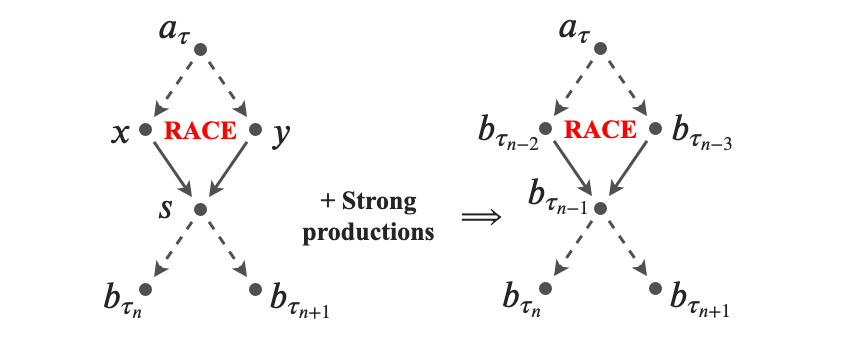
\includegraphics[width=0.48\textwidth]{pics/millwheel}
  \caption{Strong productions mechanism}
  \label {millwheel}
\end{figure}

Such behavior is also called {\em effective determinism}~\cite{akidau2018streaming}, because computations become deterministic until the persistent storage is cleared. Strong productions method guarantees that even if multiple possible results of a non-commutative operation may be obtained due to races, only one of them is actually computed and saved. The price for such exactly once enforcement technique is an overhead on external writes on each transformation in a physical graph.

\subsection{Spark streaming}

The  $\Gamma$ is a set of all possible {\em RDD} records. Unlike pure streaming engines like Flink and MillWheel, where input elements arrive one by one, RDD is a small collection of data that is atomically processed. Dependency relation on the power set of $\Gamma$ is also defined using a directed acyclic graph of user operations. Spark inherits main properties form batch processing systems including the fact that each new stage of computations is started only after the previous one is completed. 

Hence, the conditions of Theorem~\ref{necessary_conditions} are satisfied and determinism is simply achieved. Recovery function $F$ restores just the last non-complete stage.
 
To the best of our knowledge, spark streaming is the only state-of-the-art stream processing system that provides for deterministic results. However, an architecture based on the processing of collections of buffered input elements ({\em micro-batching}) makes it hard to achieve latency lower than several seconds~\cite{7530084, 7474816}. 

% \subsection{Flink}

% The  $\Gamma$ is represented as all {\em StreamRecords}. Relation $D$ is defined in the form of a directed acyclic graph consisted of user operations. Flink periodically saves information needed for recovery by injecting special elements called {\em checkpoints} into the input stream. Checkpoints go through the same network channels as ordinary elements and push all inverted dependencies of inputs through the system. Each operation prepares data to save independently at the moment of checkpoint arrival. Prepared data is committed to external storage when checkpoint passes through the whole data flow. Output elements are delivered to end-user only after the commit. This mechanism ensures that the results of non-commutative operations are saved before delivery of their dependencies that allows Flink to satisfy the Theorem~\ref{necessary_conditions}, but dramatically increases latency as we show further. Recovery function $F$ restores operation states and replays only input items which do not affect these states.

% Besides overhead on snapshotting and delivery synchronization, checkpoints cause extra latency overhead because an operation with multiple inputs must wait until checkpoints arrive from each input. Only after that, an operation can safely send checkpoint further. This behavior is known as {\em checkpoints alignment}.